\documentclass[12pt]{report}

\usepackage[left=0.75in, right=0.75in, top=0.75in, bottom=0.75in]{geometry}
\setlength\parindent{0pt}

\usepackage{graphicx, amsmath,anonchap,tabularx,multicol}
\usepackage{wrapfig}

\usepackage{enumitem}
\setlist{noitemsep}
\setlist{nolistsep}

\newenvironment{boxe}
    {\begin{center}
    \begin{tabular}{|p{0.9\textwidth}|}
    \hline\\
    }
    { 
    \\\\\hline
    \end{tabular} 
    \end{center}
    }

    \newenvironment{boxe2}
    {\begin{center}
    \begin{tabular}{|p{0.9\textwidth}|}
    \hline\\
    }
    { 
    \\\hline
    \end{tabular} 
    \end{center}
    }

\begin{document}
\begin{tabular*}{\textwidth}{@{\extracolsep{\fill}}l l}
\textbf{The Definition of the Derivative and Derivative Shortcuts} \\
MATH 160\\
%\textbf{Due Friday, 10/22/18} & MATH 157\\
\hline\hline
\end{tabular*}\\
\begin{boxe2}
\textbf{The Definition: }The \textbf{Derivative} of $f(x)$ at $x=a$ denoted $f'(a)$ or $\frac{df}{dx}|_{x=a}$ is 
\[ f'(a)=\lim_{h \rightarrow 0}\frac{f(a+h)-f(a)}{h} \]
\textbf{Interpreting The Definition: } Think of this definition as the process of 
bringing $h$ to $0$. For any $h$ in this 
process $\frac{f(a+h)-f(a)}{h}$ tells us about the slope of the secant line, or average rate of change, 
between the fixed point $(a,f(a))$ and the floating point $(a+h,f(a+h))$. 
And so this (limiting) process tells us about the AROC as the points get closer and closer, 
giving us the instantaneous rate of change, or the slope of the tangent line.
\begin{center}
    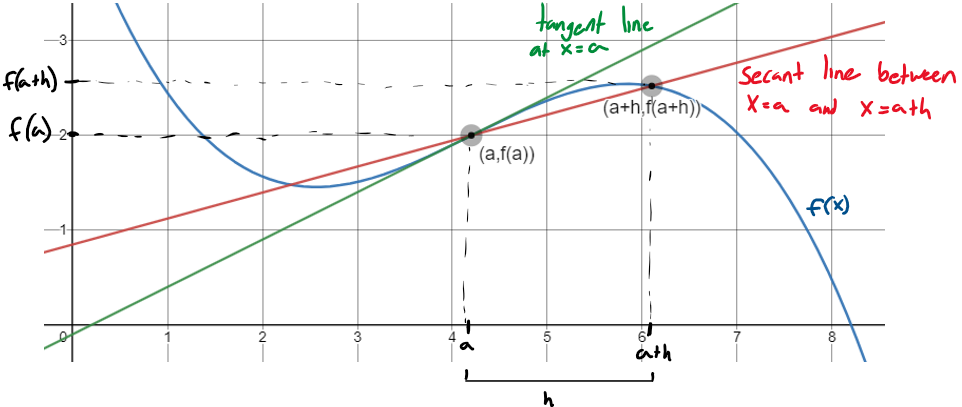
\includegraphics[scale=.6]{lim-def.png}
\end{center}
\end{boxe2}

\begin{boxe2}
\textbf{Interpreting Derivatives: } The units of a derivative function $f'(x)=\frac{df}{dx}$ are $\frac{\text{units of }f(x)}{\text{units of }x}$.\\
The derivative tells us about the instantaneous rate of change of the function $f(x)$ with respect to the input variable $x$.
That is $f'(a)$ tells us how much the $y$-values of $f(x)$ will change at $x=a$ if we move along the $x$-axis.\\\\


\textbf{Displacement: } If $r(t)$ tells us about a displacement 
(Ex. the distance, in meters, a biker is from the engineering building after $t$ seconds) 
Then the derivative function $r'(t)=\frac{dr(t)}{dt}$ tells us the rate at which the biker is moving away from (in the positive direction) or towards (in the negative direction) the engineering building.
That is $r'(t)$ tells us about the velocity $v(t)$, in meters per second, of the biker.\\\\
\textbf{Graphically:} The derivative tells us when a graph is increasing/decreasing and the second derivative tells us about the curvature
\begin{center}
\begin{tabular}{c|c|c}
    $f(x)$ & $f'(x)$ & $f''(x)$\\
    \hline
    Increasing & $f'(x)>0$ & \\
    Decreasing & $f'(x)<0$ & \\
    \hline
    Concave Up & Increasing & $f'(x)>0$\\
    Concave Down & Decreasing & $f'(x)<0$ \\

\end{tabular}
\end{center}
\end{boxe2}
\section*{Derivative Shortcuts}
\begin{boxe}
    \textbf{Power Rule: } If $n$ and $a$ are numbers:\\
    $\displaystyle{\frac{d}{dx}\left[ax^{n}\right]=anx^{n-1}}
    \;\;\;\;\;\;\;\;
    \displaystyle{\frac{d}{dx}\left[a \right]=0}$\\
    \textbf{Exponent Rule: } If $a$ is a number:\\
    $\displaystyle{\frac{d}{dx}\left[a^x\right]=\ln(a)a^x}
    \;\;\;\;\;\;\;\;
    \displaystyle{\frac{d}{dx}\left[e^x \right]=e^x}$\\

    \textbf{Log Rule: } if $a$ is a number:\\
    $\displaystyle{\frac{d}{dx}\left[\log_a(x)\right]=\frac{1}{\ln(a)x}}\text{ , for }x>0
    \;\;\;\;\;\;\;\;\;\;\;
    \displaystyle{\frac{d}{dx}\left[\ln(x)\right]=\frac{1}{x}}\text{ , for }x>0$\\

    \textbf{Trig Rules: }\\
    $\displaystyle{\frac{d}{dx}\left[\sin(x) \right]= \cos(x)}\;\;\;\;\;\;\;\;\; \displaystyle{\frac{d}{dx}\left[ \cos(x)\right]= -\sin(x)}\;\;\;\;\;\;\;\;\;\displaystyle{\frac{d}{dx}\left[\tan(x) \right]= \sec^2(x)}$\\
    \vspace{.05pt}
    $\displaystyle{\frac{d}{dx}\left[ \csc(x)\right]= -\csc(x)\cot(x)} \;\;\;\;\;\;\;\;\;\displaystyle{\frac{d}{dx}\left[ \sec(x)\right]= \sec(x)\tan(x)}\;\;\;\;\;\;\;\;\; \displaystyle{\frac{d}{dx}\left[ \cot\right]= -\csc^2(x)}$
    \end{boxe}

    \begin{boxe}
        If $f$ and $g$ are differentiable functions and $a$ a constant then\\
        \textbf{Coefficient Rule: } $\displaystyle{\frac{d}{dx}\left[af(x) \right]=a\frac{d}{dx}\left[f(x) \right]=af'(x) }$\\
        \textbf{Sum/Difference Rules: } $\displaystyle{\frac{d}{dx}\left[f(x)\pm g(x) \right]=\frac{d}{dx}\left[f(x) \right]\pm \frac{d}{dx}\left[g(x) \right]=f'(x)\pm g'(x) }$\\
        \textbf{Product Rule: } $\displaystyle{\frac{d}{dx}\left[f(x) g(x) \right]=\frac{d}{dx}\left[f(x) \right]g(x)+ f(x)\frac{d}{dx}\left[g(x) \right]=f'(x)g(x)+ f(x)g'(x) }$\\
        \vspace{.1pt}
        \textbf{Quotient Rule: } $\displaystyle{\frac{d}{dx}\left[\frac{f(x)}{g(x)} \right]=\frac{f'(x)g(x)- f(x)g'(x) }{(g(x))^2}=\frac{g(x)f'(x)- f(x)g'(x) }{(g(x))^2}}$\\
        ``lo di hi minus hi di lo, draw the line, and square below''\\
        \textbf{Chain Rule: } $\displaystyle{\frac{d}{dx}\left[f(g(x)) \right]=f'(g(x))\cdot g'(x)=\frac{df}{dg}\cdot\frac{dg}{dx}}$
\end{boxe}



\end{document}
